\chapter{統計モデル}

\section{正規分布を含んだ統計モデル}
\begin{quote}
    \begin{enumerate}[(1)]
    \item 独立同分布
    \item その分布は、正規分布
    \item 正規分布の母数(平均と分散)はそれぞれ$\mu,\sigma^2$。
    \end{enumerate}
\end{quote}
データを大文字の$X_1,X_2,\cdots,X_n$とし、モデルからサンプリングした確率変数を小文字の$x_1,x_2,\cdots,x_n$とする。

\subsection{データが出現しやすい区間}
ある決められた確率でデータが出現するとモデルが予測する区間を予測区間という。
割合として、よく使われる$95\%$を設定したものを$95\%$予測区間という。
正規分布を含んだモデル$M(\mu)$において、予測区間は比較的簡単に求めることができる。
具体的には、正規分布の規格化を行い、標準正規分布に従うように変換を行い、$\frac{x-\mu}{\sigma}$であるので、予測区間は、
\begin{eqnarray*}
    -z_{0.05} <\frac{x-\mu}{\sigma} <z_{0.05} \\
    \mu-z_{0.05}\sigma < x < \mu+z_{0.05}\sigma
\end{eqnarray*}
である。この範囲にデータが生じることをモデルが予測する。

\subsection{平均値が出現する区間}
今回考えている統計モデル$M(\mu)$では、次の統計量$Z$が標準正規分布$N(0,1)$に従うことが、正規分布の再生性によってわかっている。
$$
Z(\bar{X},\mu)=\frac{\sqrt{n}(\bar{X}-\mu)}{\sigma} \sim N(0,1)
$$
ここで$\bar{X}$は、統計モデル$M(\mu)$からサンプリングした標本の標本平均値(データの平均値ではない)、$\mu,\sigma$は統計モデルで設定した母数平均、母数分散。
$Z(\bar{X},\mu)$が$N(0,1)$に従うということから、$Z(\bar{X},\mu)$が$N(0,1)$における出現頻度が計算できる。
\begin{figure}
    \begin{center}
        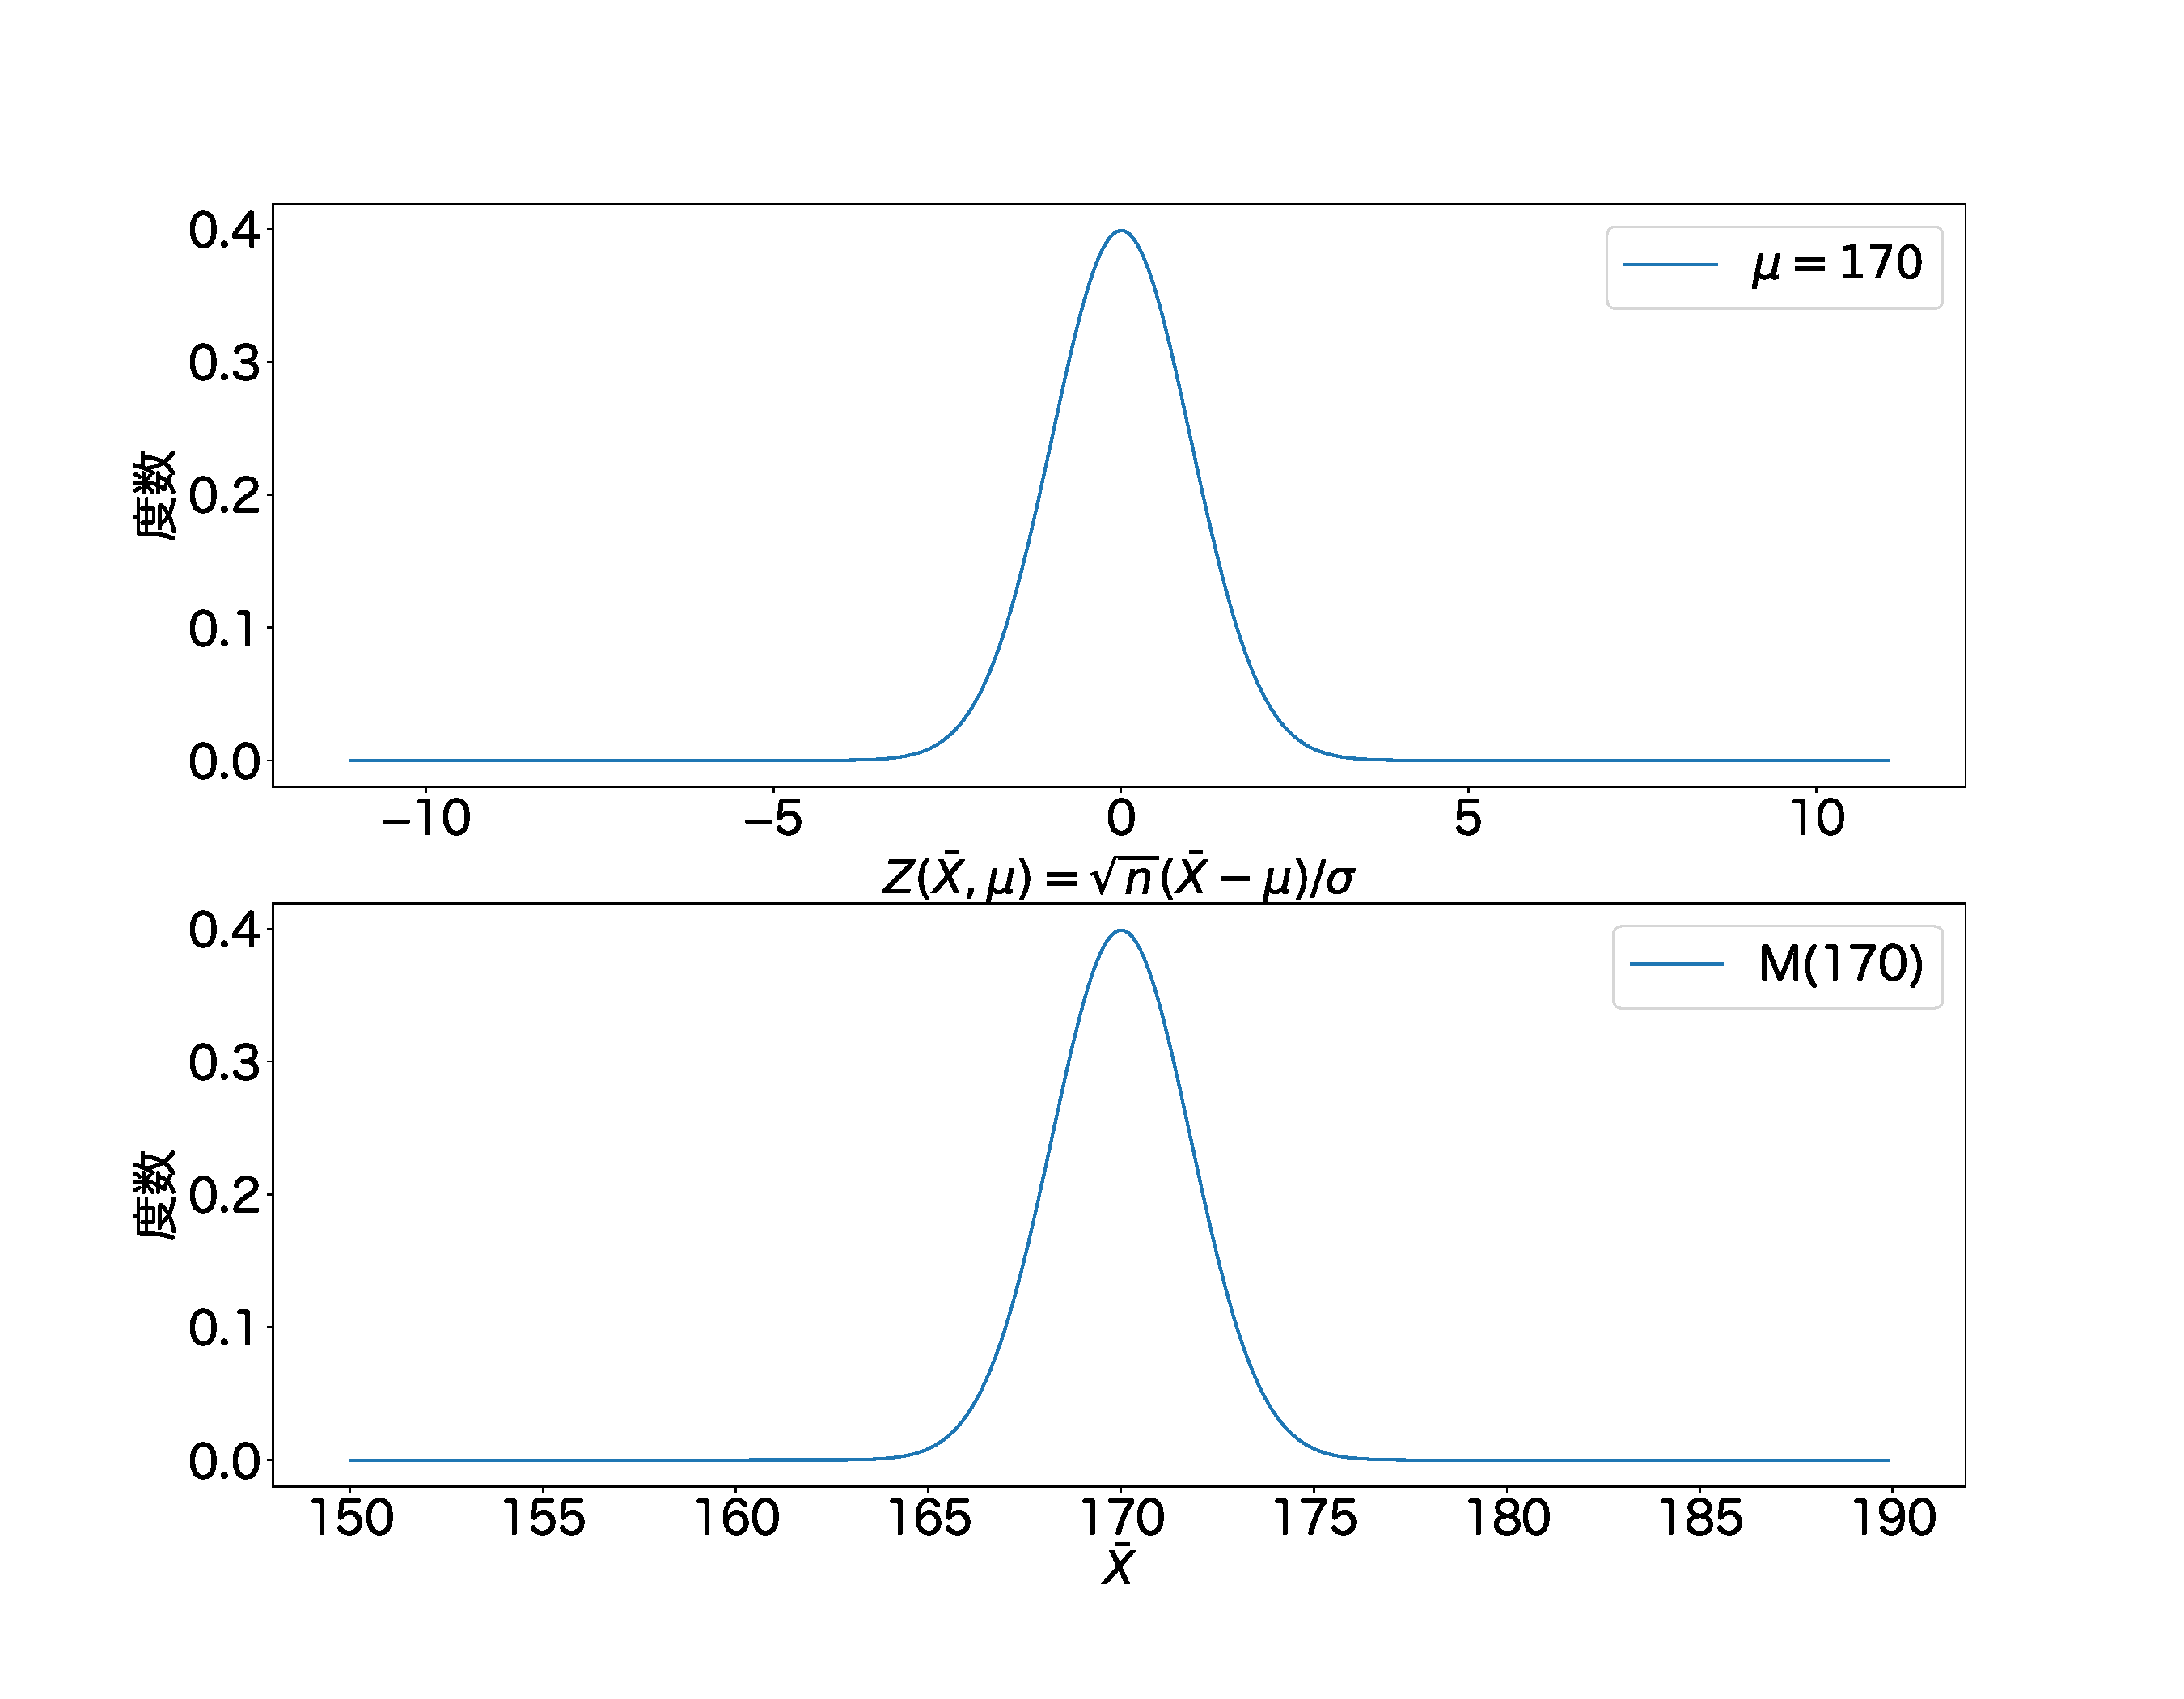
\includegraphics[width=15cm]{./image/03_/normal_Z_frequency.pdf}
        \label{fig:cm_standard_normal_distribution}
      \end{center}
    \end{figure}

$Z$の出現頻度を$Z$または$\bar{X}$の値に応じて書いたものが図\ref{fig:cm_standard_normal_distribution}です。
$Z(\bar{X},\mu)$の$95\%$予測区間が次のように求められる。
$$
-z_{0.025}<Z(\bar{X},\mu)<z_{0.025}
$$
このの範囲で、サンプリングされた標本の統計量$Z(\bar{X},\mu)$が$95\%$の確率で得られる。
統計モデルを使った判断でよく出てくる確率として分野を問わず、$95\%$が使われる。
%この値には身長に関する経験を使わずに決定しています。


$Z(\bar{X},\mu)$を式変形することで、標本平均が$95\%$の確率で出現する区間が推定できる。式を変形する。
\begin{eqnarray*}
    & -z_{0.025} < Z(\bar{X},\mu)<z_{0.025} \\
\rightarrow & -z_{0.025} < \frac{\sqrt{n}(\bar{X}-\mu)}{\sigma}  <z_{0.025} \\
\rightarrow & \mu - z_{0.025} \frac{\sigma}{\sqrt{n}} < \bar{X} < \mu + z_{0.025} \frac{\sigma}{\sqrt{n}}
\end{eqnarray*}
この統計モデルからサンプリングした標本の標本平均$\bar{X}$が$95\%$の確率で見つかる範囲のことを$95\%$信頼区間という。

\subsection{サンプルサイズによる影響}
式を見てわかるように、サンプルサイズ$n$が大きくなれば、$\bar{x}$が入る範囲は狭くなる。
信頼区間がサンプルサイズに依存することを数値的に確認する。
図\ref{fig:confidence_interval_n}は、信頼区間が$N$に応じて変化する様子を図示している。

\begin{figure}
\begin{center}
    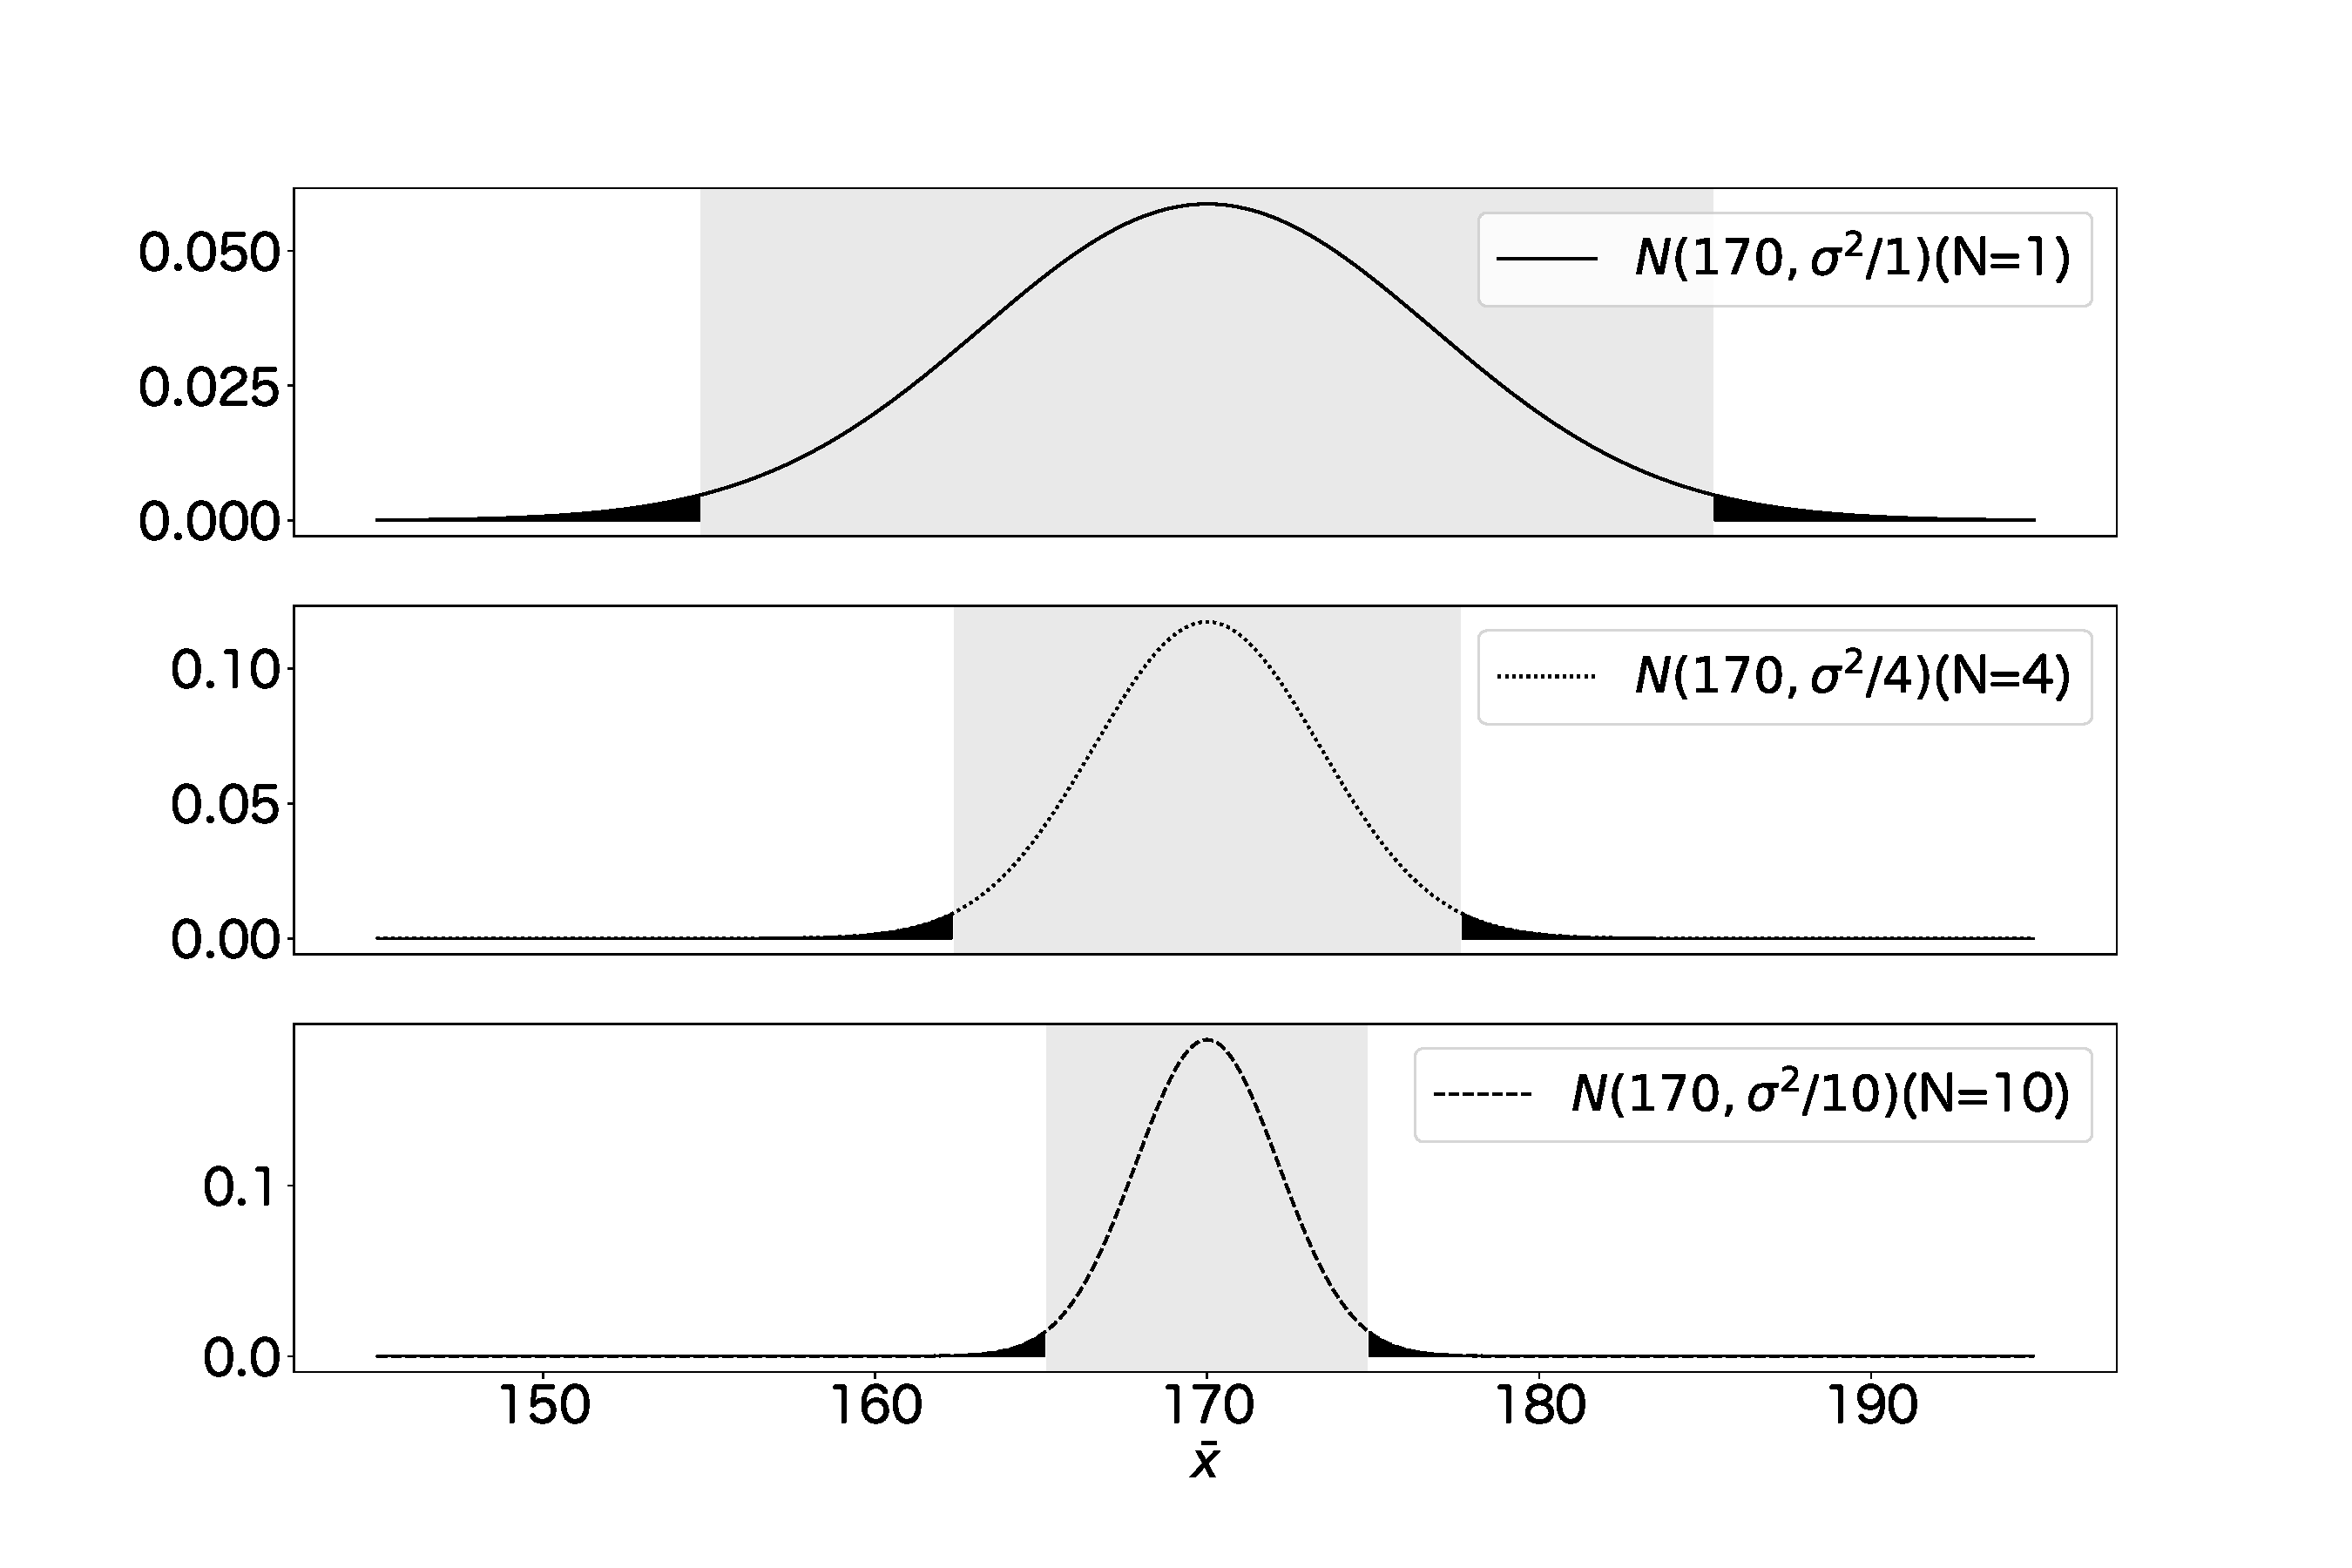
\includegraphics[width=15cm]{./image/03_/confidence_interval.pdf}
%    \caption{信頼区間}
    \caption{(A)$N=1$,(B)$N=4$,(C)$N=10$での信頼区間}
    \label{fig:confidence_interval_n}
  \end{center}
\end{figure}


\begin{framed}
    まとめ、
    \begin{itemize}
        \item 統計モデル$M(\mu)$によってサンプリングし、標本を得たとき、標本平均値のよくある値の範囲が信頼区間
    \end{itemize}
    \end{framed}
    


\section{標本が統計モデルにより生成されたのかを判断する方法}%統計モデルの性質を使った方法}
%ここまでは、統計モデルの予測がデータと一致することを定量的に評価した。
ここでは、推測に適していないと判断する方法である、統計的仮説検定を紹介する。
この方法は、統計量の一つである統計検定量の統計モデル上での出現しやすさにより、モデルを評価する。

\if 0
 川久保統計学P.166
 \fi


%![Z値の頻度]()

信頼区間の中に標本平均が含まれていることは、標本がモデルにり推測可能であることの証拠の一つになる。
ただし、証拠の一つであり、このことは実際には複合的に指標を見て判断する必要がある。
%$\bar{X}$が$95\%$信頼区間の中に入っていることは、この統計モデル
%信頼区間の中に統計量があれば、
%このことから、統計モデル$M(\mu)$でサンプリングしたときに、$95\%$の確率で、この範囲に平均値$\bar{X}$がえられます。


%標本$1$標本$2$について、これを計算してみる。平均値は、それぞれ172.4, 169.0です。
\if 0
標本では、$168.9 < \mu < 176.0$、
この範囲にある$\mu$をもつ統計モデルであれば、この標本によって棄却されない。
%標本$2$では、$165.5 < \mu <172.6$です。
例えば、このモデル$M(\bar{x})$の信頼区間であれば、$M(168)$は棄却できない。
\fi


まとめ、
\begin{framed}
    \begin{itemize}
        \item 統計モデル$M(\mu)$のサンプルの平均が$95\%$の確率で入る範囲$\mu - z_{0.025} \frac{\sigma}{\sqrt{n}} < \bar{X} < \mu + z_{0.025} \frac{\sigma}{\sqrt{n}}$。現実の母集団が統計モデルによってよく推測できるなら、この範囲に平均値が入る確率は$95\%$に近くなることもある。逆に、統計モデルが現実をよく捉えることができなければ、母集団から無作為抽出した標本の平均値はこの範囲に入ることは少なくなる。
        \item データがよくある範囲に入る統計モデル$M(\mu)$の$\mu$の範囲$\bar{x}- z_{0.025}\frac{\sigma}{\sqrt{n}} < \mu < \bar{x} + z_{0.025}\frac{\sigma}{\sqrt{n}}$
        \item  統計モデル$M(\mu)$ではサンプルサイズを大きくすると、平均値が入る範囲が狭くなる。
    \end{itemize}
\end{framed}



\section{最尤推定量を使ったモデル}


母集団から無作為抽出した標本を元にモデルを構築する。具体的には、$\mu=\bar{x}$とし、統計モデル$M(\bar{x})$をモデルにする。これを最尤モデルと呼ぶ。
\if 0 
このモデルにおいて、統計量$Z(\bar{x},\mu)$の$95\%$予測区間を求める。
%よく入る区間の式を変形し、データを得たときに、そのデータを基準にした$\mu$の範囲に変形してみます。
\begin{eqnarray*}
 & -z_{0.025} < Z(\bar{x},\mu)<z_{0.025} \\
\rightarrow & -z_{0.025} < \frac{\sqrt{n}(\bar{x}-\mu)}{\sigma}  <z_{0.025} \\
\rightarrow & \bar{x}- z_{0.025}\frac{\sigma}{\sqrt{n}} < \mu < \bar{x} + z_{0.025}\frac{\sigma}{\sqrt{n}}
\end{eqnarray*}
\fi

\if 0

\section{問題意識}
確率変数$x_1$または、$x_1,x_2,\cdots,x_n$を得たとき、それらが独立同分布に従うという前提のもと、ある母数をもつ分布関数に従う、または従わないと推測することは可能であるだろうか。
最尤推定から、確率変数を得たなら、最尤推定を行って、母数を推測可能な場合がある。
具体的には、正規分布から得られた確率変数については、その平均と分散は、$(\mu,\sigma^2)=(\bar{x},\sum_{i=1}^{n} (x_i-\bar{x})^2/n)$である。

この問題に対して、
正規分布から確率変数を得たとき、ある母数平均$\mu$をもつ正規分布からサンプリングされていないということはできるだろうか。これを議論する。




\subsection{問題点}
aa



\fi
\section{指数分布を含んだ統計モデル}
指数分布における信頼区間は式\ref{exp_model_confidence_interval}である。

\subsection{中心極限定理により信頼区間を近似する}

\section{モデルの比較}
